\documentclass[twocolumn]{revtex4}
\usepackage{graphics,graphicx,epsfig,amsmath,multirow,gensymb,commath,textcomp,natbib,blindtext,mhchem,tabularx,array,makecell,threeparttable,amssymb,relsize}
\usepackage[a4paper, left=1.85cm, right=1.85cm, top=1.85cm, bottom=1.85cm]{geometry}   
\usepackage[normalem]{ulem}
\newcommand{\squeezeup}{\vspace{-2.5mm}}

\def\bibsection{\section*{\refname}} 
\renewcommand{\thesubsection}{\alph{subsection}}

\renewcommand\theadalign{bc}
\renewcommand\theadfont{\bfseries}
\renewcommand\theadgape{\Gape[4pt]}
\renewcommand\cellgape{\Gape[4pt]}

\begin{document}

\textheight=26.385cm
%Change textheight as the last resort...

\title{Observing Type Ia supernovae and fitting templated light curves}
 
\author{Jacky Cao, AstroLabs Michaelmas, Lab Partner: Duncan Middlemiss \\ Dates of experiment: 19/10/2017 to 08/12/2017, Date of report: 07/01/2018}

\begin{abstract}              
We have measured the magnitude of supernova explosions over an extended period of 34 days using a $16''$ and a $0.5$ m telescope situated in Durham and La Palma. We have plotted several light curves and have identified a Type Ia and Type Ia-91bg supernova, 2017hhz and 2017hle. With our data we have fitted template light curves with the Python routine, \textit{SNooPy}. These fittings have produced reduced $\chi^2$ values in the B and V bands of 1.68 and 2.78 for 2017hhz, and 1.29 and 3.02 for 2017hle. This indicating that the fittings are good in the V band but really good in the V band. We expect our biggest source of uncertainty arose due to the conditions and data analysis that we performed. Using a Type Ia supernova of brightness $00.00$ mag, we have managed to produce a value for Hubble's Constant, $H_0 = 74$ kms$^{-1}$ Mpc$^{-1}$. We attempted to calculate Einstein's coefficient, $\Lambda$, but this was unsuccessful due to redshift of something.
\end{abstract}

\maketitle

\vspace{-3ex}
\section{Introduction} 
\label{intro}
\vspace{-2ex}
In astronomy, one of the most violent and luminous events which can occur are supernova explosions. At the end of a massive star's lifetime, as a star runs out of nuclear fuel to burn, there is a possibility that the equilibrium configurations for a star will cease to exist. This leads to a final cataclysmic event, a supernova explosion. The luminosity of such, when at it's peak, can be as bright as a small galaxy \cite{longair}.

Observing these events and measuring their magnitude over a period of time allows us to plot light curves. The likes of which can then be used to visualise the evolution of a supernova. Using these plots we can draw the conclusion that there is order in the explosions. We find that if our sample of supernovae is large enough, we see that they can be grouped together into different types just by features from their light curves. The two general types of supernova are Type I and Type II, the difference between them being that Type I lacks the Balmer hydrogen features in it's spectra \cite{longair}, and that Type II events are very hydrogen-rich \cite{obs_phys_class_sn}.

\vspace{-3ex}
\subsection{Supernovae Classification}
\vspace{-2ex}

If we were to further study the light curve shapes and also the spectra of the supernovae from our sample, we would begin to recognise that there are further sub-classifications within Type I and Type II. In Table \ref{sn_classes} some of these subtypes are specified.

\begin{table}[h!]
\centering
\begin{tabular}{c@{\hskip 20pt}c} 
 \hline
 \textbf{Type} & \textbf{Characteristic} \\ 
 Ia		& Si II line present at $616.0$ nm in spectra \\
 Ia-91bg	& Absorption trough at $400-450$ nm in spectra \\
 		& \em Type Ib and Type Ic also exist \em \\
 IIP 		& Reaches a plateau in it's light curve  \\
 IIL		& Rapid linear decrease in light curve \\
 		& \em Type IIn and Type IIb also exist \em \\
 \hline
\end{tabular}
\caption{Some of the subclassifications of supernova and their respective characteristics which distinguish between them from each other \cite{longair, obs_phys_class_sn}.}
\label{sn_classes}
\end{table}
\squeezeup

In the application to cosmology, one of the most used types of supernovae are Type Ia, their light curve profiles are generally homogenous which allows them to be used as standard candles, thus providing a reliable distance indicator.  

We can see this homogeneity in Figure \ref{typeia-standard}. This plot was produced by superimposing and translating multiple sets of Type Ia data. The light curves in the B and V bands (further discussion on bands and photometric filters in Section \ref{observer-collection}) follow a general path in their evolution: they initially increase in brightness until they reach a peak magnitude, after this point the magnitude of the supernova decreases until no noticeable change can be detected by our telescopes. We note that whilst Type Ia's do peak at different magnitudes in when observed from in different bands, it is not as pronounced as is shown in Figure \ref{typeia-standard}.

\squeezeup
\begin{figure}[!h]
\begin{center}
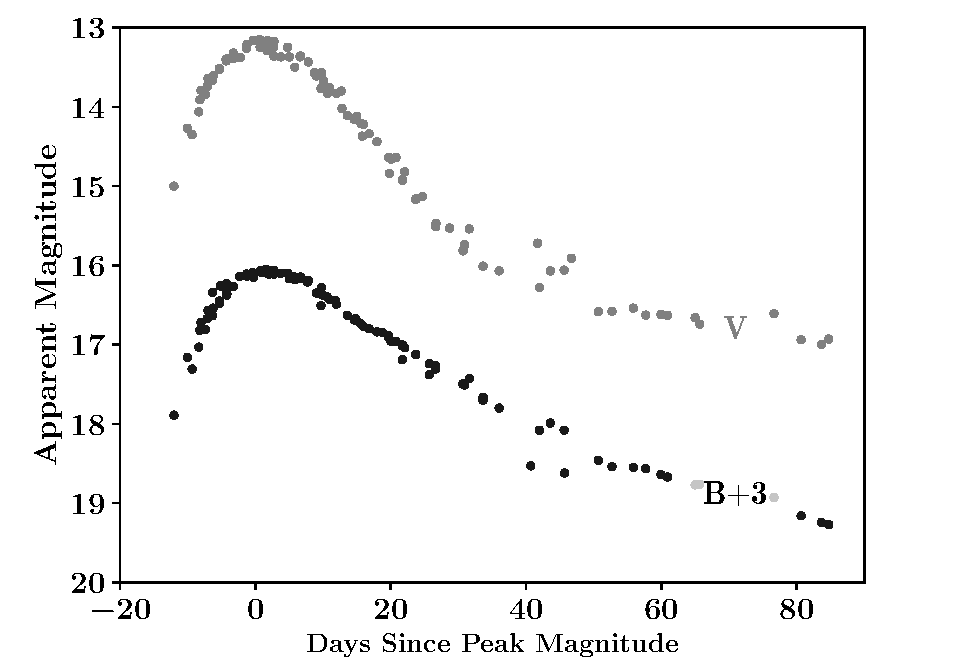
\includegraphics[width=9.25cm]{intro/typeia}
\caption[]{Plot showing the general forms of Type Ia supernovae in the B and V bands. Archival data was translated along the time axis and magnitude axis to produce the general forms of the light curves. The B band has been offset by a magnitude of $3$ to allow us to see both graphs clearly. The supernovae which were used to plot this graph are: \em{1994ae, 1994S, 1995bd, 1996bo, }\em  and \em{1998aq }\em \cite{jha, matheson}. }
\label{typeia-standard}
\end{center}
\end{figure}
\squeezeup
\squeezeup

In understanding the consistency of Type Ia light curves, we must attempt an exploration of the mechanisms of the explosion. This will involve developing an understanding of the system pre-supernova and also post-explosion.

The general consensus for Type Ia pre-supernova, as discussed by B. W. Carroll and D. A. Ostlie \cite{mod_ast}, is that a white dwarf within a binary system accretes matter from a donor star. However, this is also the initial system for dwarf novae and classical novae, which can grouped together as cataclysmic variables or novae. These too increase in brightness (classical novae by a factor of $\sim 10^6$ \cite{mod_ast}) which can lead to some confusion with supernovae, especially if you observe them optically without following up with any spectroscopic observations. 

It is understood that the difference which leads to cataclysmic variables and Type Ia supernovae is the process of accretion. This is dependent on the binary companion star, if the secondary star is on the main sequence then the white dwarf would just be steadily burning hydrogen or helium in it's surface layers, thus we would have a cataclysmic variable. To produce a supernova explosion we require a progenitor star to increase in mass towards the Chandrasekhar limit of $1.4$ $M_{\odot}$ \cite{posn, longair}. 

If the primary white dwarf was to accrete matter continually from it's binary companion until it itself was brought close to and past the critical mass, then a collapse to a neutron star must occur. However for a Type Ia supernova explosion this is not the case, before the collapse, the star is disrupted by large amounts of energy due to fusion reactions.

We can attribute this energy release to the fusion of carbon and oxygen within the core of the white dwarf. As material is continually accreted and compressed onto the surface, the star is heated and the temperature increases to $T \geq 10^9$ K \cite{longair}. When the thermonuclear energy is released, the white dwarf loses it's electron degeneracy pressure, and so becomes gravitationally unstable \cite{longair}. However, this energy that is produced disrupts the star and prevents the total collapse into a neutron star, this disruption leads to a supernova explosion \cite{posn}. 

In performing spectroscopic observations of Type Ia supernovae at maximum light we see that intermediate mass elements such as silicon, calcium, magnesium, sulphur, and oxygen are present which supports the picture of thermonuclear disruption \cite{longair, mod_ast}.

The process continues until the heaviest element that nuclear fusion can produce is made, iron. This is created from nickel capturing an electron through electron-capture (ec) into cobalt, and then the cobalt captures an electron and $\beta^{+}$ decays into iron \cite{mod_ast}. The process can be summarised in the following equation:
\begin{equation*}
\ce{^{56}Ni} \xrightarrow{\text{ec}} \ce{^{56}Co} \xrightarrow{\text{ec, $\beta^{+}$}} \ce{^{56}Fe}.
\end{equation*}

With these processes, they can be used to explain the form of the Type Ia light curves. The luminosity at peak maximum can be explained as the energy which has been deposited into the expanding envelope from the decay of the \ce{^{56}Ni} nuclei \cite{mod_ast}. We can highlight other features as seen in Figure \ref{typeia-standard}: the increase to peak magnitude is a fast process, it increases roughly half a magnitude a day; and the maximum of the light curve can be approximated as a Gaussian function \cite{mod_ast}. 

However, there are some peculiar types of Type Ia supernovae. For example, as featured in Table \ref{sn_classes}, Type Ia-91bg are a class of supernovae which have spectra which resembles those of Type Ia, however, they have an absorption band at $400-450$ nm. This arises due to a blend of Fe-group elements which is dominated by Ti II \cite{obs_phys_class_sn}. With their light curves they also lack the secondary maximum as found in normal Type Ia's within the I and R bands.

Observing objects and recognising that they are Type Ia supernovae thus requires not only spectroscopic observations but also observations in the optical. 

\vspace{-3ex}
\subsection{Supernova Discovery}
\vspace{-2ex}
In attempting to discover supernovae it is important that the search is not confined to a single region of the sky, whilst it may be possible to discover one of these events within that region, it would perhaps take a very long time until you could actually witness and collect data on it. What is thus required is a survey which spans the entire sky. 

A general method which can be employed to discover new supernovae is one which involves data comparison. If a survey takes an image of the entire night sky for every night, then to find new supernovae all that would be required is to subtract one night's data from the previous' and any objects which remain would be objects that could be new supernovae \cite{assasn-rev}. In reality it is not that simple, frames need to be cleaned of noise and they also require to be transformed in response to the point spread function. Plus, follow up observations would have to be made to verify if the object is supernovae or whether it is an anomalous object such as a cataclysmic variable. 

One such survey which employs this is the \em{All-Sky Automated Survey for Supernovae }\em (or ASAS-SN). Built up of five observations stations around the world, they produce a coverage of around $48,000$ square degrees of the night sky and they allow us to see up to a depth of $\sim 17$ mag \cite{asn_lc}, ASAS-SN is able to find many more supernovae and also supernovae which are close to the cores of galaxies, vastly increasing the discovery rate of bright supernova explosions and improving our understanding of where these events occur.

However, the majority of the supernovae are close enough to the detection limit that they need to be validated by other astronomers \cite{asn_lc}. This human review of transients has led to projects such as \textit{Supernova Hunters} \cite{cit-sci}, a citizen science program where volunteers are asked to classify objects which could be potential supernova candidates.  

These programs do not detract from the work that astronomers have to perform in the classification of supernovae, but it is equally important as it allows for the improvement of neural networks so that automatic surveys such as ASAS-SN could work more autonomously and efficiently \cite{cit-sci}.  

\vspace{-3ex}
\subsection{Application to Cosmology} \label{appcosmo}
\vspace{-2ex}
Once optical observations for Type Ia supernovae have been obtained, light curves can then be produced - the conversion of a time series of photometric observations into a set of model parameters for each supernova \cite{sn_consts}, this can then be used for cosmology. 

We find that before Type Ia supernovae data has been corrected for the correlation between maximum luminosity and the width of the light curve about maximum luminosity \cite{longair, abs_phil}, the dispersion of the absolute magnitudes at peak is less than 0.5 magnitudes. Once this correlation is accounted for, there is little dispersion and the light curves lie on top of one another, they are homogeneous in nature. 

With this in mind, if a new Type Ia supernova is discovered and enough data has been collected to produce a light curve, using that and the width-luminosity relation it would be possible to calculate their absolute magnitudes, thus they can be used to determine the redshift-distance relation \cite{mod_ast}.

For example, if we had a sample of nearby Type Ia supernovae with redshifts of $\mathrel{\mathsmaller{\lesssim}} 0.1$, we could derive a value for Hubble's Constant by plotting them on a Hubble diagram \cite{exp_uni_sn}, and in turn use a rearranged form of Hubble's Law,
\begin{equation}
H_0 = \frac{v}{d}, 
\label{h_nought}
\end{equation}
where $H_0$ is the value for Hubble's Constant, $v$ is the recessional velocity of the supernova, and $d$ is the distance to the supernova \cite{mod_ast}. 

To calculate the recessional velocity, the redshift of the supernova has to be obtained, this could be obtained by making spectroscopic observations of the supernovae, and then $v$ would be calculated using,
 \begin{equation}
v = zc,
\label{redshift}
\end{equation}

where $v$ is the recessional velocity of the supernova, $z$ is the redshift of the supernova, and $c$ is the speed of light in a vacuum \cite{mod_ast}.

Extending the usage of Type Ia's in cosmology, they could also be used to provide statistical constraints on cosmological models, for example for an $\Omega_M$, $\Omega_{\Lambda}$ Universe (where $\Omega_M$ is the mass density which includes ordinary and dark matter, and $\Omega_{\Lambda}$ is the effective mass density of dark energy) \cite{mod_ast, exp_uni_sn}. Additionally, the time-averaged equation of state of dark energy, $w$, could be measured \cite{sn_consts}. This is a value which can be used to characterise the state of the universe - for an accelerating, dark energy dominated universe we would find that $w \approx -1$ \cite{longair}. 

We thus find that Type Ia supernovae are a useful tool which can be applied and used within cosmology.

\vspace{-3ex}
\subsection{Project Aims}
\vspace{-2ex}
This paper discusses the study that was undertaken to observe Type Ia supernovae using ground based telescopes, to learn about the approaches which can be employed to fit template light curves onto collected data, and to evaluate these analytical methods.

In Section \ref{obsver} we describe how we collected and analysed our supernova data, and how we accounted for the uncertainties that arose during the experiment. Our final light curves, and the methods that were used to fit models to the observations is summarised in Section \ref{analysis}. Then in Section \ref{discussion} we further discuss the model fitting, primarily our usage of the fitter program, \textit{SNooPy}, we then discuss the usage of our data for supernova cosmology, and finally we analyse the methods and techniques which we employed to produce our light curves and we explore the potential work that could be performed.

%We also focussed on understanding the sources of uncertainties and attempted to reduce them within our analysis to produce magnitudes which would be more true to what they should be [[?]]. 

%From collected data it would be possible to produce light curves which we can use to identify the type of supernova that we were observing. In also understanding the uncertainties further analysis could be performed such as galaxy subtraction or [[think of something for here...]].

\vspace{-3ex}
\section{Observations} 
% Write in past tense!
\label{obsver}
\vspace{-2ex}
\subsection{Data Collection}
\label{observer-collection}
\vspace{-2ex}
To observe supernova explosions our main pieces of experimental equipment were telescopes which had been fitted with CCD cameras.

We employed three out of the four telescopes based on the Department of Physic's Roof in Durham, and also the robotic telescope on the roof of the William Herschel Telescope building at Roque de los Muchachos Observatory in La Palma.

For the vast majority of our observations we used the 16$''$ telescope (Far-East-16, or FE16) from the Durham array and the robotic 0.5 m telescope (pt5m) from La Palma. We used these two telescopes predominantly as they allowed us the best resolution and illumination on our faint objects. Compared to the 14$''$ telescopes which are also part of the Durham array, having a larger aperture means that a more sufficient number of photons could be obtained so that we could study our targets more clearly. 

Both Far-East-16 and pt5m are variants of the Cassegrain Telescope, they are Ritchey-Chr\'{e}tein Telescopes. This derivative is composed of a hyperboloidal primary and secondary mirror \cite{tel_tech} as can be seen in Figure \ref{cassegrain}. With this design, the telescope can produce good quality images over a field of view of several tens of arcminutes across as opposed to just a few minutes of arc when a basic Cassegrain design is used \cite{tel_tech}. 
\squeezeup
\begin{figure}[!h]
\begin{center}
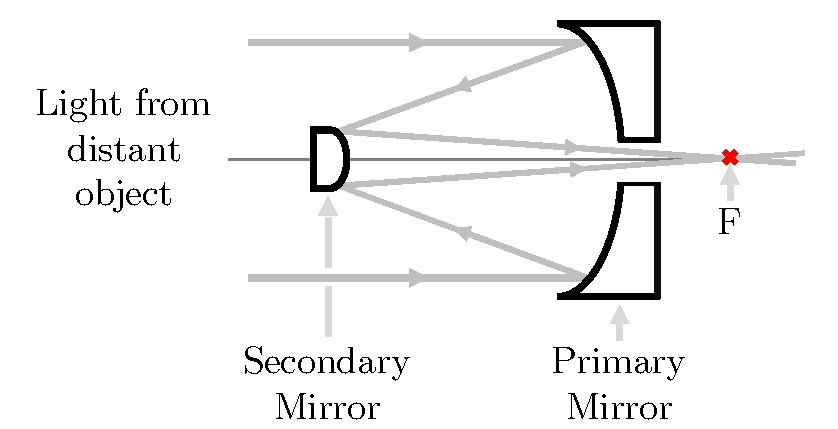
\includegraphics[width=7.5cm]{observations/cassegrain}
\caption[]{A schematic overview of a Cassegrain/Ritchey-Chr\'{e}tein Telescope, in the former design the primary mirror is paraboloidal, and in the latter the primary mirror is hyperboloidal. In both types of telescope the secondary mirror is a convex hyperboloidal and F is the focal point of the telescope where a CCD camera can be placed. \\ (\textit{This diagram has been adapted from Telescopes and Techniques} \cite{tel_tech}.)}
\label{cassegrain}
\end{center}
\end{figure}
\squeezeup
\squeezeup

To record and make use of the collected light from our supernova targets we had to use CCD cameras which were mounted at the focal points of our telescopes. On Far-East-16, a QSI 583ws CCD was used with an LX200R telescope, and with pt5m a Kodak KAF-3200ME CCD with an Officina Stellare 0.5m Ritchey-Chr\'{e}tein telescope. In a simplified manner, these CCD cameras would convert the photons into electrons and then the electron signal would be processed by a computer into an image \cite{mod_ast, tel_tech}. This could then be manipulated and analysed using software packages such as \textit{GAIA} \cite{starlink}.

For our project in particular, we wanted to produce light curves of supernovae within different colour bands. By using photometric filters on our CCDs we were able to observe supernovae within these bands. Meaning that we were only able to view specific wavelengths of light from our objects, this would correspond to particular energies in the elements present in astronomical bodies \cite{astro_filters}. 

Once we had selected our observation filters and began observations, we had to be acutely aware of the possible over-saturation of the CCDs. As our objects were faint and observing conditions could often be bad, we had to collect as much light as possible before our images became oversaturated due to a brighter object within the same field of view. This would be mitigated by lowering the time that we would be observing for, thus there would be less photons collected from the secondary object.

In spite of this, having just one image of our faint supernovae to analyse would not be representative of it's magnitude. Through the process of image stacking (more in Section \ref{observer-observations}) we were able to improve the quality of the image by compositing together several images of the same area of sky. Thus it was beneficial during our observation nights to take multiple exposures for our chosen given exposure time and also for each photometric filter that we were going to use. 

As we progressed through our experimental period we came to realise that astronomical observations are heavily reliant on weather conditions. What happened to be occurring in the atmosphere that night would have an influence on what you could see with your telescope. This overall effect of the atmosphere on images is called \textit{seeing} \cite{tel_tech}.

In the first instance, having a night sky without any visible clouds would be a good initial step. Once the conditions appear to be clear, the atmospheric turbulence would have to be considered next. This is the process when air is turbulently mixed together at different temperatures, thus creating cells or pockets which have different refractive indexes when compared to their surrounding area \cite{princ_stell_inter}. The effect of this is to produce an image which is blurred and appears to have moved.

In quantifying this seeing as a value, the full width at half maximum (FWHM) can be given for each observation made. The FWHM is a resolution criterion which can be defined as, $``$the diameter of the Airy disk at half of its maximum intensity'' \cite{princ_stell_inter}. The Airy disk being the central spot of the diffraction pattern which occurs when light from a distant point source has been diffracted by a circular aperture, say, by a telescope. 

Given in arcseconds, the best observing sites produce a stellar image about $0.25''$ across, for an average site it will be typically $2''$ \cite{tel_tech}. What we found was that for Far-East-16, our seeing ranged from $3''$ on a clear night to $\sim6''$ on a cloudy and turbulent night. For pt5m, we found that seeing was generally better on good nights as it is in a better location for astronomical observations. [[why]]

Then to account for atmospheric turbulence, one could use an adaptive optic system to correct for the distortions. For example, an artificial laser guide star could be created and then the amount that it is being perturbed by can be applied to the main object that is being observed \cite{princ_stell_inter}.

However, as Far-East-16 and pt5m are not equipped to perform these measurements, these disturbances could not be accounted for by us. As a result of this, we had to choose nights when the wind was calm, and at times the telescopes had to be refocussed to adapt to the changing atmosphere.

We note that this latter solution was only possible when we were observing in Durham (and not La Palma) as the CCD settings could be manually altered on the fly from the Durham control room.

During our observations bad seeing due to changing weather conditions was not the only factor which would affect us and which we could not account for. Light pollution is a common problem in astronomy and we were no exception to it. With Far-East-16, as the telescope is elevated onto the Department of Physics' roof, the light pollution from the majority of the City of Durham could be avoided. Our problems arose when our objects were in the night sky above Durham Cathedral. This historic building uses spotlights to illuminate parts of itself, some of this light inevitably bleeds off into the sky which creates a halo of light, something not beneficial for magnitude based observations.

Similarly, if our targets were within $40\degree$ or less to the Moon on the celestial sphere, then observations would not be possible as the reflected sunlight would create a disc of light and drown out the supernovae. This effect would especially be magnified if the Moon was in a Full Moon phase.

We thus find that there are multiple factors which we have to be aware of and also consider when performing our observations. From the types of photometric filters to weather conditions, there are multiple factors which contribute to the final data set that we collect.

\vspace{-3ex}
\subsection{Observations Made}
\label{observer-observations}
\vspace{-2ex}
Over a period of 34 days we made observations of 19 different objects, some Type Ia supernovae, a few Type II, and some cataclysmic variables. These objects are noted in our objects log in Appendix A, and our individual observations from the entire experiment are detailed in Appendix B.

It was realised early on in our project that it would not feasible for us to track multiple objects for an extended period. This was firstly because observation time had to be distributed equally amongst all the projects within AstroLabs, it would be unfair to observe just supernovae for the entire night; secondly with such a large amount of data, we would not be able to process and analyse it all; and thirdly, some of the targets were just not worth observing at all. These objects would be too close to their host galaxy, or they would be too low on the horizon for the telescopes in Durham or La Palma to view them.

In choosing which objects to observe we used the \textit{Rochester Bright Supernova} \cite{rochester_sn} and \textit{ASAS-SN Supernovae} \cite{asassn_sn} Lists. These are databases which are updated by astronomers with the latest discovered supernovae. For our observations we aimed to choose supernovae which had a discovery magnitude of around 18 or less, anything greater than this would be too faint to observe with our telescopes.

After reviewing and considering which objects would provide the best basis for producing Type Ia light curves, we chose two supernovae targets, 2017hhz and 2017hle, a Type Ia and Type Ia-91bg respectively. Both being not too close to their host galaxy's nucleus and they appeared to the brightest supernova objects discovered at the time.

However, they were still faint objects so we had to vary the exposure time between 60s and 120s, and often take more than 2 exposures for each band. In doing so we would later be able to improve the quality and brightness of the supernovae seen in the image through noise reduction and image stacking.

\vspace{-3ex}
\subsection{Data Analysis} \label{data_analysis}
\vspace{-2ex}
As data was continually collected over the experimental period, we had to simultaneously analyse it to ensure that the magnitudes we were obtaining would fit supernova light curves.

Photometry was thus performed on each of our frames. Our goals were to: take our supernova images, reduce unwanted noise, and then obtain a magnitude value with a related uncertainty. After this, we could use these values in template fittings, and then attempt to perform cosmology.

Taking our raw frames we had to reduce the noise from unwanted sources. Two sources which we did not have to consider directly was the bias and dark current. The bias arises due to the readout of a CCD, it creates noise when it is converting the captured signal from analogue to digital \cite{obs_uni}. To account for this, bias frames of zero second exposures are taken and subtracted from the data before the data is stored. On the other hand, dark current is the creation of electrons due to the thermal energy of the CCD, these electrons would be read as a signal \cite{obs_uni}. However, the chips are normally cooled to about $-10\degree$ to prevent any such noise from forming.

The CCD produces one other type of noise which can be account for, each pixel on the CCD varies slightly from each other in terms of sensitivity, something which arises due to the manufacturing process. This sensitivity is normally removed by producing frames of a uniformly lit area, flat-fields. The twilight sky or the inside of the telescope dome can be imaged, and this can then be subtracted from our data.
 
Cosmic rays which register onto the camera can be removed by stacking (combining) multiple frames of the same field and same exposure time together. This is a process where the median value for each pixel is found from the stack of images, thus any anomalously high values which arise from cosmic rays can be removed.

Once our frames had been cleaned of noise we could then begin to perform photometry, more specifically, aperture photometry. After identifying the supernova in our images, we then wanted to calculate the absolute magnitude of it and see how it progressed with time. To perform this we had to choose at least two calibration stars, of which they had to be of similar size to the supernova and be in the general proximity of it.  This was so that when performing aperture photometry a similar signal could be obtained across all objects and a similar sky background noise could be obtained as well. Noise which arose from the night sky and which could not be directly removed through subtraction techniques.

Another important criterion for these calibration objects is that their absolute magnitudes must already be known. This was required in the calculation of the magnitudes for the supernova. So, we used the \textit{UCAC4 Catalog} to find the photometric data for the calibration stars in the B and V bands. For the 2017hhz frames we chose calibration stars 512-002598 and 512-002599, and for 2017hle we used 613-003374 and 613-003367. These names are the identifiers used by UCAC4. Once we had our data and calibration stars, we could use the following equation, 
\begin{equation}
    m = z - 2.5 \log_{10}{C},
\label{mag_counts}
\end{equation}

where $m$ is the absolute magnitude of an object, $z$ is the zero-point of the frame, and $C$ is the number of counts we receive from the object.

In using this equation we first required the zero-point for the image that we were working with. What we imaged would not be the actual magnitudes of the objects, they would be offset by a certain amount, $z$, due to light being absorbed by dust in the supernova's host galaxy, through the interstellar medium, and by the dust that is in our own galaxy.

To begin with then, the counts $C$ for the calibration stars were measured, with this and the absolute magnitudes $m$ we could solve equation \ref{mag_counts} for $z$. Once this was done for each star within each required band, the $z$ values could then be all averaged together within their respective observation bands. This zero-point could then be used with the number of counts for the supernova to produce an absolute magnitude value for the supernova.

With obtaining a value for the counts, whether from the supernovae or from the calibration objects, we had to choose a fixed aperture size to count the signal that was contained within in, and a fixed sky annulus to count the sky background noise. It was important that the radius of both the aperture and annulus would maximise the signal whilst reducing the amount of sky noise measured.

This was done by selecting one of the calibration stars and then plotting how the signal-to-noise ($S/N$) ratio would change as the radius was increased. Derived from High Energy Astrophysics \cite{longair}, we used the following equation for the signal to noise,
\begin{equation}
\frac{S}{N} = \frac{N_{\gamma}}{\sqrt{N_{\gamma}+N_{b}+N_{d}+R^2}},
\end{equation}

where $N_{\gamma}$ is the supernova signal, $N_{b}$ the sky background noise, $N_{d}$ the noise due to dark current, and $R$ the readout noise. The latter two sources of noise were reduced and could be ignored in our calculations.

In Figure \ref{2017hhz_radii}(a) we show the $S/N$ plot that was created for the 2017hhz frames, the calibration star (512-002599) was selected from the V band data from the 20th October 2017 as it appeared to have the least noise.
\squeezeup
\begin{figure}[!h]
\begin{center}
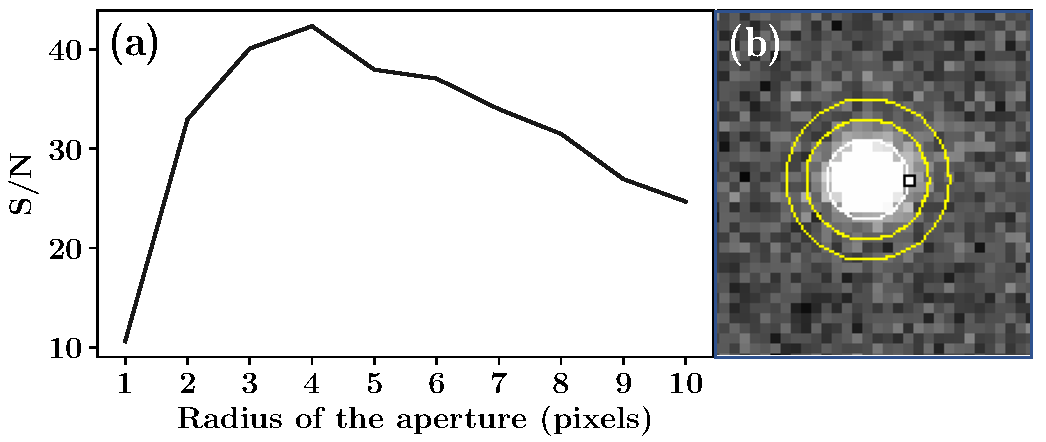
\includegraphics[width=8.5cm]{observations/2017hhz}
\caption[]{(a) Plot of signal to noise against the radius of the aperture for 2017hhz frames, this was used to identify which fixed radius to use. (b) Image of the aperture tool used: inner white circle around star is the main aperture, the outer yellow annuli is used to measure the sky background. Object shown is star, 512-002599.}
\label{2017hhz_radii}
\end{center}
\end{figure}
\squeezeup
\squeezeup

The point where the plot decreases was chosen to be the radius as this would produce an optimal value for the signal to noise. In the case for 2017hhz this was chosen to be 4 pixels and for 2017hle it was 3 pixels. 

Figure \ref{2017hhz_radii}(b) shows the aperture tool that was used extensively for the aperture photometry. With the white circle as the main aperture that we varied, and the two outer yellow circles being the sky annuli. The area enclosed in the sky would be�sampled and then as quantified amount of noise, it would be removed away from the main counts value. The size of these rings were chosen as the radius scaled by factors $\times 1.5$ and $\times 2$. These numbers were justified as we wanted to avoid taking other stars as part of the sky background, and whilst this did mean we had to take part of the galaxy when we were working with our supernovae, we chose to be consistent with our calibration stars as it was difficult to balance just having sky in each individual annuli.

For the placements of these apertures, we took a histogram profile of the vertical and horizontal directions of the object, and then placed the centre of the aperture to the centre of the maximum brightness. 

After we had calculated magnitude values we could then proceed to plot supernova light curves with our data, the process of which can be found in Section \ref{supernovae_models}.

\vspace{-3ex}
\subsection{Data Uncertainties}
\vspace{-2ex}
Throughout the experiment it was important that we kept in mind the uncertainties which could affect the accuracy of our results. Various steps were undertaken to ensure that the sources of errors could be reduced, some of these methods have already been detailed in Section \ref{data_analysis} however we would like to discuss other random and systematic uncertainties.

In collecting data, we have already learnt how a CCD could count extra noise in the form of bias and dark current if it is not accounted for. Alternatively, we found that as our Type Ia supernovae progressed along their evolutionary path we found that as they continually dimmed, it became increasingly difficult for us to produce a precise result. This random error is a result of the observational limits of the telescopes, as they could only observe to a certain magnitude it would be expected that the magnitudes produced would have a larger uncertainty.

Having access to a larger telescope, one with a greater aperture would allow us to collect more light and thus produce a more accurate and precise value for the supernova magnitudes.

If we consider the systematic errors of our experiment, the greatest source would be as a result of our aperture photometry. Whilst we tried to ensure that we used a set method and set conditions, we may still have accidentally misplaced the positioning of one of the apertures. 

We chose to perform the photometry manually, however to reduce the potential systematic error, we should have automated the process with a script. In doing so, we would be more certain that the counts and magnitudes that we obtained would be more accurate to the true value of the magnitude of the supernova.

On the other hand, we could have repeated the photometry and then took an average value for the counts to reduce any random and systematic errors which may occur. However, as we tried to ensure that our apertures were on the position of peak brightness of their respective objects, hopefully it would make no difference. 

\vspace{-3ex}
\subsection{Final Data}
\vspace{-2ex}
Tables \ref{2017hhz-table} and \ref{2017hle-table} contain the calculated magnitudes with their associated uncertainties. We note again that Equation \ref{mag_counts} was used for the magnitude, and Equation \ref{m_uncert} for the uncertainty. From this we could then plot Type Ia supernova light curves and then attempt to perform cosmology with the results.

\begin{table}[h!]
\centering
\begin{tabular}{c@{\hskip 20pt}c@{\hskip 20pt}c@{\hskip 20pt}c@{\hskip 20pt}c} 
 \hline
 \textbf{Date Observed} & \textbf{$\boldsymbol{m_B}$} & \textbf{$\boldsymbol{\Delta{m_B}}$} & \textbf{$\boldsymbol{m_V}$} & \textbf{$\boldsymbol{\Delta{m_V}}$} \\ [0.5ex] 
 20/10/17 & 16.8 & 0.1 & 17.1 & 0.1 \\
 22/10/17 & 16.9 & 0.1 & 16.8 & 0.1 \\
 23/10/17 & 16.8 & 0.2 & 16.9 & 0.1 \\
 26/10/17 & 17.0 & 0.2 & 17.0 & 0.1 \\
 29/10/17 & 17.2 & 0.1 & 17.0 & 0.1 \\
 30/10/17 & 17.3 & 0.1 & 17.1 & 0.1 \\
 05/11/17 & 17.7 & 0.2 & 17.3 & 0.2 \\
 11/11/17 & 18.2 & 0.4 & 17.5 & 0.2 \\
 16/11/17 & 18.6 & 0.2 & 17.8 & 0.1 \\
 17/11/17 & 18.8 & 0.2 & 18.2 & 0.4 \\
 \hline
\end{tabular}
\caption{10 days worth of data was analysed to produce magnitudes and their uncertainties for the B and V photometric bands for Type Ia supernova, 2017hhz. }
\label{2017hhz-table}
\end{table}

\begin{table}[h!]
\centering
\begin{tabular}{c@{\hskip 20pt}c@{\hskip 20pt}c@{\hskip 20pt}c@{\hskip 20pt}c} 
 \hline
 \textbf{Date Observed} & \textbf{$\boldsymbol{m_B}$} & \textbf{$\boldsymbol{\Delta{m_B}}$} & \textbf{$\boldsymbol{m_V}$} & \textbf{$\boldsymbol{\Delta{m_V}}$} \\ [0.5ex] 
 26/10/17 & 17.8 & 0.3 & 16.8 & 0.1 \\
 29/10/17 & 18.4 & 0.2 & 17.0 & 0.1 \\
 30/10/17 & 18.6 & 0.2 & 17.1 & 0.1 \\
 16/11/17 & 19.5 & 0.3 & 18.9 & 0.2 \\
 17/11/17 & 19.3 & 0.4 & 18.7 & 0.3 \\
 18/11/17 & 19.6 & 0.5 & 18.7 & 0.3 \\
 \hline
\end{tabular}
\caption{6 days worth of data was analysed for the Type Ia-91bg supernova, 2017hle. For the B and V band, their magnitudes are shown with their associated uncertainties.}
\label{2017hle-table}
\end{table}

\vspace{-3ex}
\section{Analysis}
\label{analysis}
\vspace{-2ex}
\subsection{Supernovae Models}
\label{supernovae_models}
\vspace{-2ex}
In fitting templates and models to our data, the process could be manually performed, however we chose to use a Python package \textit{SNooPy} \cite{car_snoopy}. SNooPy is an automated fitter for Type Ia light curves, our magnitudes would be parsed and then a template would be transformed to fit that set of data. 

For the basic fitting function, \texttt{snpy.fit()}, it would only work if we provided a set of data in at least two different photometric bands out of the passbands of uBVgriYJHK. SNooPY also required a right ascension and declination of the supernova in order for it calculate the galactic extinction from Schlegel maps \cite{snoopy_docs}. On top of that, a value for the heliocentric redshift of the supernova was also needed for the fitting, this is because it is required for the computation of the K-corrections in each of the filters provided \cite{car_snoopy}. 

The redshift values for our supernovae were obtained from the discovery notes that were attached to their entry's on the Rochester Bright Supernova List. As our objects were Type Ia they generally would be of interest for cosmology, spectroscopic observations would thus often be performed after their initial discovery, and so we could use the redshift that they obtained.

After it had managed to apply the template light curves, this fitting could then be exported and plotted. In addition to this, the final parameters that had been selected by SNooPy could be obtained as well. These included the host galaxy extinction (EBVhost), the time for B-maximum (Tmax), the distance modulus to the supernova (DM), and the decline-rate parameter (dm15). Values which would be useful to us when we attempted to perform some cosmology.

To see the correlations between these four parameters, covariance plots could be produced using the \texttt{fitMCMC()} function with the argument \texttt{plot\_triangle} selected as \texttt{True}. A covariance matrix with the values could be retrieved and then potentially plotted to produce a heat map as an alternative to the triangle plots. 

A full example of how SNooPy was used has been provided in Appendix C.

\vspace{-3ex}
\subsection{Results}
\vspace{-2ex}
After running our data through SNooPy, we were able to produce Type Ia light curves with the \texttt{fit()} function for 2017hhz and 2017hle. In Figure \ref{2017hhz-lc} and Figure \ref{2017hle-lc} we show the respective light curves, their plotted magnitudes and their uncertainties for the the B and V bands.

In Table \ref{chi2-table} the $\chi^2$ and reduced $\chi^2$ statistics have been calculated for both supernovae, and for both B and V bands.

Figure \ref{covar-plots} shows some of the covariance plots produced by \texttt{fitMCMC()} in SNoopy displaying the correlation between the time for B-maximum, the host galaxy extinction, the distance modulus, and the decline-rate parameter.

With Figure \ref{2017hhz_collage} two samples of our data, a frame of our analysed data, and one of our extension projects are shown together as a collage of  images.

\begin{figure}[!h]
\begin{center}
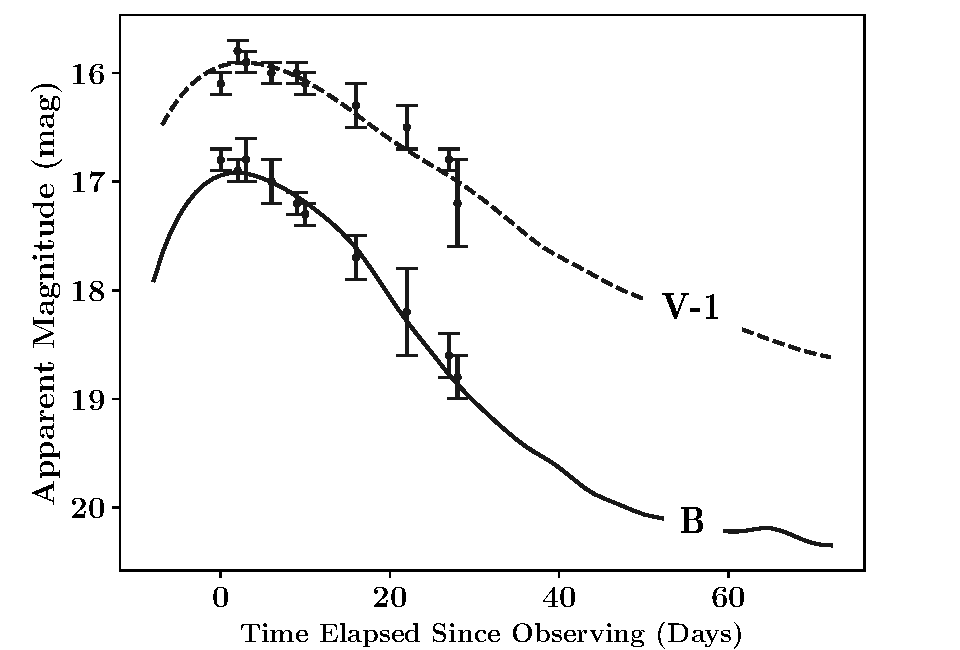
\includegraphics[width=9.25cm]{results/2017hhz}
\caption[]{Plot showing the light curves fitted by SNooPy for supernova 2017hhz. The raw magnitude data has been plotted with their uncertainty in the B and V photometric bands - the V band has been offset by 1 to more clearly show both sets of data. The zero position on the $x$- axis represents the first observation made on Friday 20th October 2017.}
\label{2017hhz-lc}
\end{center}
\end{figure}

\begin{figure}[!h]
\begin{center}
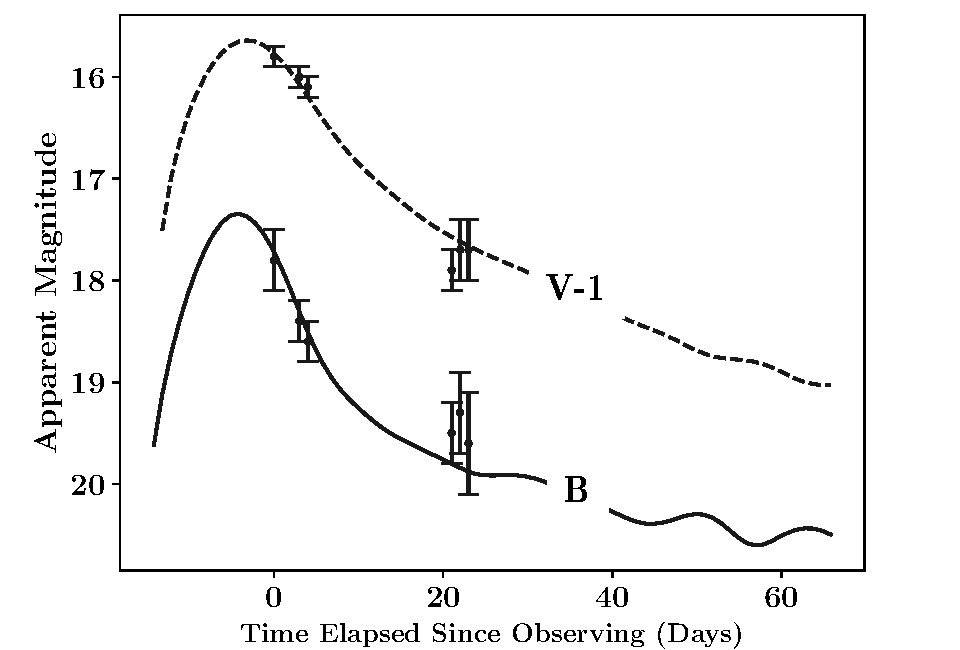
\includegraphics[width=9.25cm]{results/2017hle}
\caption[]{The calculated magnitude and uncertainties for the supernova 2017hle has been plotted along with the SNooPy fitted light curve for the B and V bands. The set of data for the V band has been offset by 1 to produce a clearer plot. Thursday 26th October 2017 represents the zero point on our $x$- axis.}
\label{2017hle-lc}
\end{center}
\end{figure}

\begin{figure}[!h]
\begin{center}
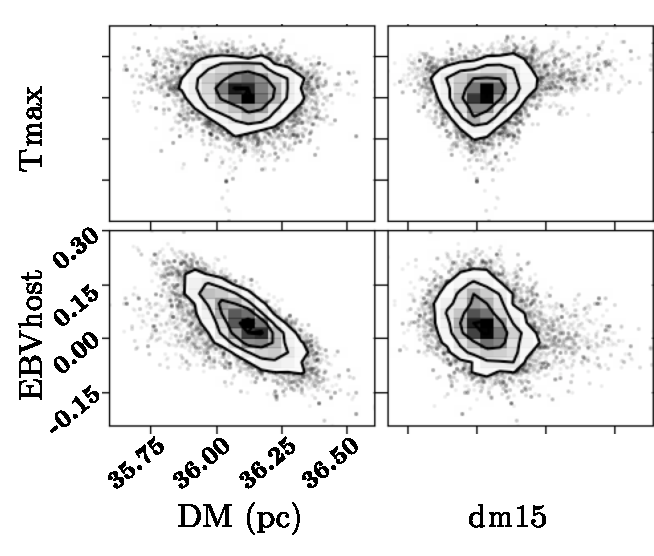
\includegraphics[width=7.5cm]{results/covariance/covariance}
\caption[]{Four out of the six covariance plots produced by the \texttt{fitMCMC()} function in SNooPy for supernova 2017hhz. The plots show the correlations between four parameters: Tmax, the time for B-maximum; EBVhost, the host galaxy extinction; DM, the distance modulus; and dm15, the decline-rate parameter.}
\label{covar-plots}
\end{center}
\end{figure}

\begin{table}[h!]
\centering
\begin{tabular}{c@{\hskip 20pt}c@{\hskip 20pt}c@{\hskip 20pt}c@{\hskip 20pt}c} 
 \hline
 \textbf{Supernova} & \textbf{$\boldsymbol{\chi^2_B}$} & \textbf{$\boldsymbol{\chi^2_{B,\nu}}$} & \textbf{$\boldsymbol{\chi^2_V}$} & \textbf{$\boldsymbol{\chi^2_{V,\nu}}$} \\ [0.5ex] 
 2017hhz & 5.03 & 1.68 & 8.23 & 2.74 \\
 2017hle & 3.86 & 1.29 & 9.05 & 3.02 \\
 \hline
\end{tabular}
\caption{$\chi^2$ and reduced $\chi^2$ ($\chi^2_{\nu}$) values are shown for each photometric filter used in our observations (B,V) for each of our supernovae, 2017hhz and 2017hle.}
\label{chi2-table}
\end{table}

\begin{figure}[!h]
\begin{center}
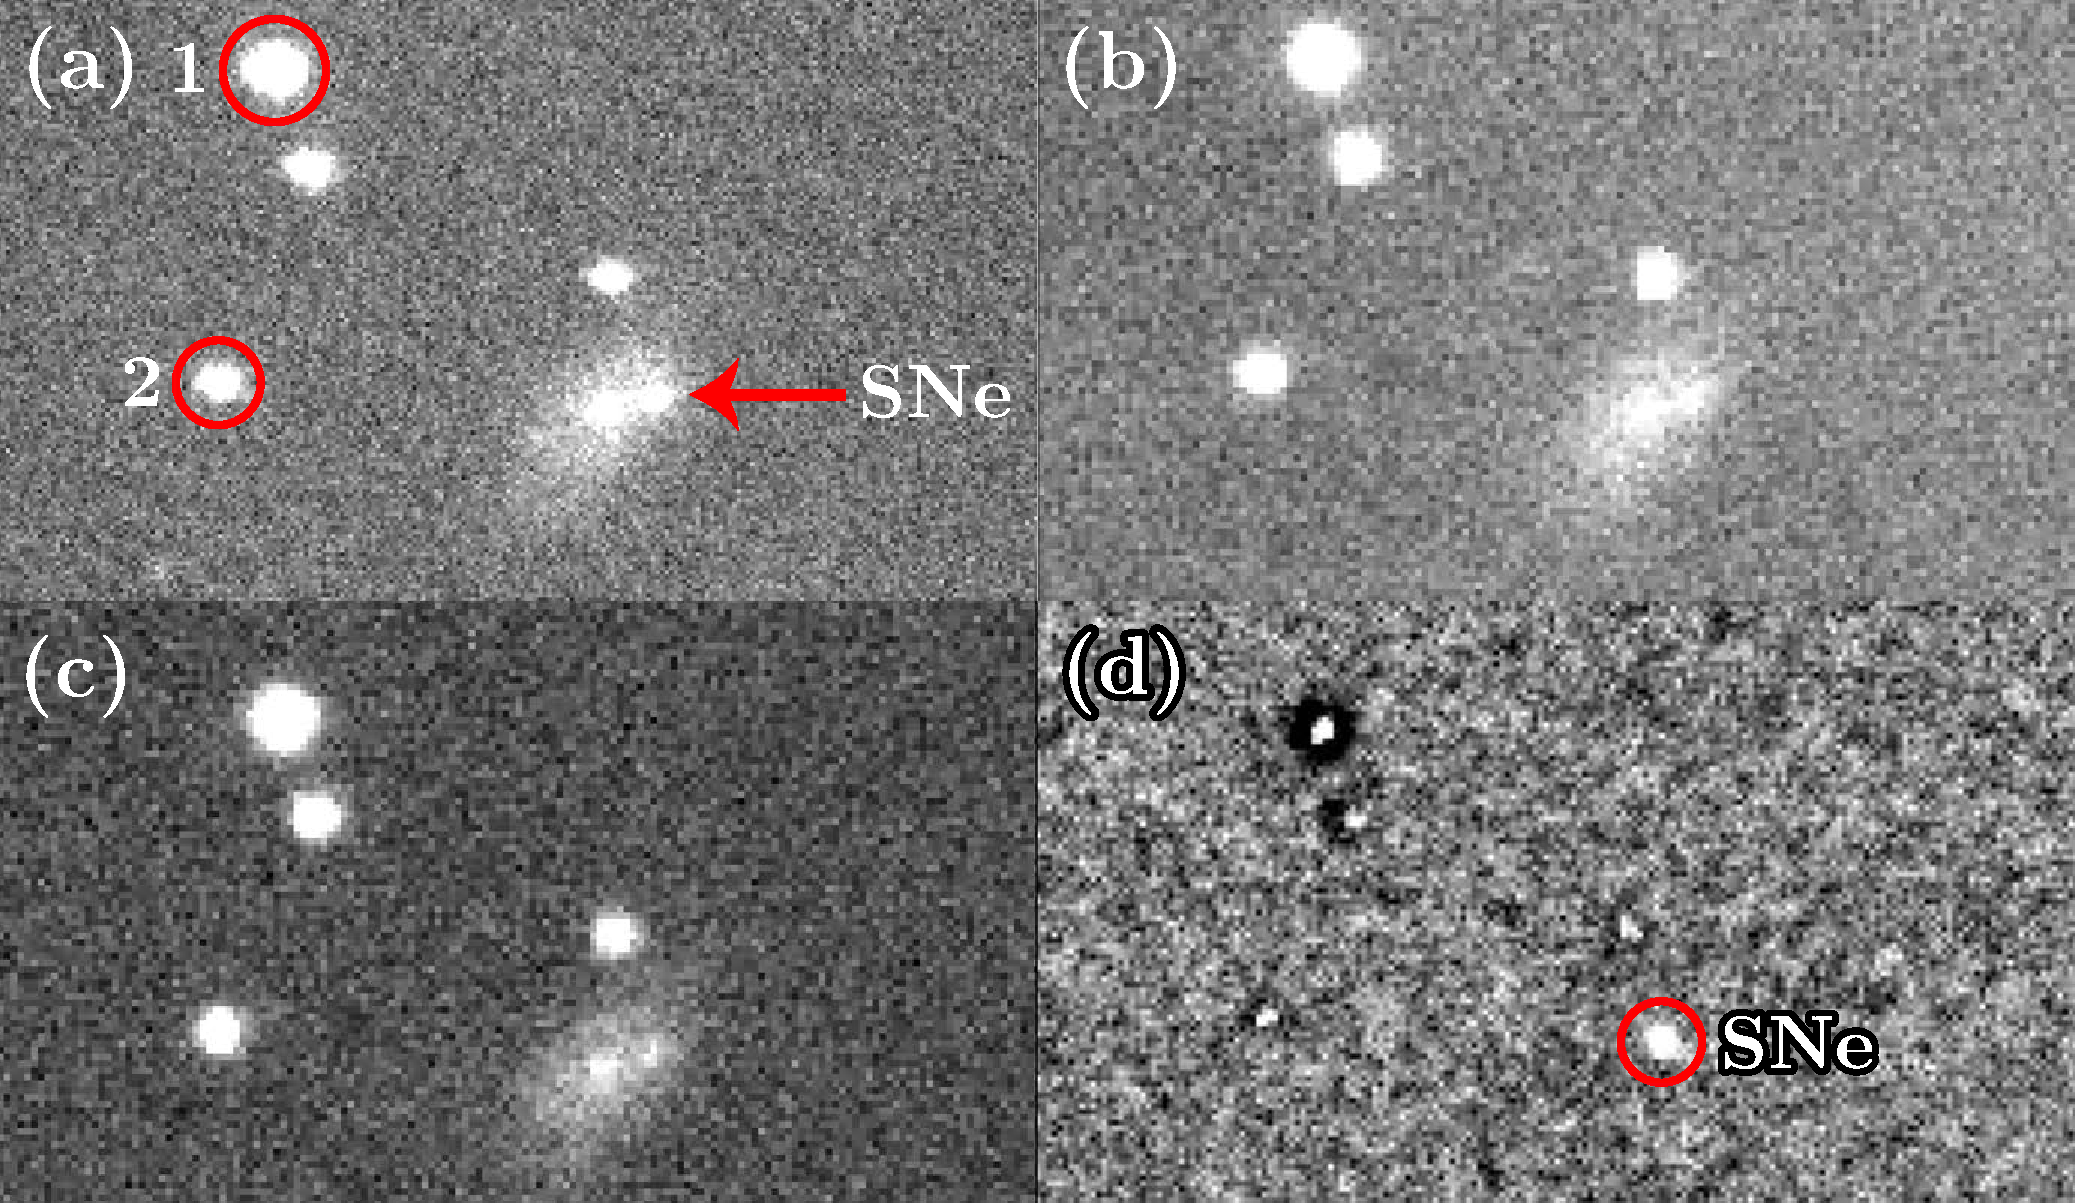
\includegraphics[width=8.25cm]{images/collage_rectangle_small}
\caption[]{Images of the supernova 2017hhz, it's host galaxy, and the stars in the same field in the V band. (a) Our first frame for this supernova from the 20th October 2017. Supernova 2017hhz has been labelled as SNe, and our calibration stars, 512-002598 as 1, and 512-002599 as 2. (b) Our last frame of data taken on 23rd November 2017. (c) Data from 23rd November 2017 when flat-fielded. (d) An attempt was made as an extension project to remove the background galaxy for the data from 20th October 2017, supernova 2017hhz has been labelled for your convenience.}
\label{2017hhz_collage}
\end{center}
\end{figure}

\vspace{-3ex}
\section{Discussion}
\label{discussion}
\vspace{-2ex}

\subsection{Using SNooPy to fit templates to supernovae}
SNooPy uses the Levenberg-Marquardt least-squares fitter to fit the model to the data [[cite]]. 

\subsection{Observing supernovae}
sdasd

\subsection{Supernovae in cosmology}

It is highly unlikely that we will see supernova remnants for the supernova that we have been studying, in the shape of the Crab Nebula. Much longer time periods would be required for this. 

In observing objects which are so faint we have the problem of trying to observe them. We need to balance the observing time to ensure that we do not oversaturate our frame with other stars. From the databases that we use, for this observation period the majority of our objects had been around the magnitudes of $\sim 18$ mag. But, we do not achieve this magnitude as there are various factors such as extinction affectinb data collection. 

We can calculate the limitiing magnitude that our telescopes could detect by analysing our frames

[neutrino studying]?



in using snoopy, how does it really fit the models to the data, what kind of parameters does it constrain. what is it's reliance on different parameters

try and produce some sort of covariance relation plot?

performing incorrect photometry and how that affects our results - not realising that we had to set a zero point, then having to find the zero point ourselves. 

confusion in observations, novae, cataclysmic variables 

there are other scripts which provide an automated way in finding the zero points from the data. what would this produce? why would this be beneficial to use this as opposed to our method?

justification of using the uncertainty equation, functional approach, why not use the uncertainty that was provided by the software? mention how it's one of the photon statistics things.

dstack, taking the median not mean , and why this is better - if I haven't discussed this already

what science have we addressed? well, we have limitations on the telescopes in terms of how 'deep' we can see:  the limiting magnitude, how that was calculated - longer exposure times...etc

has it been possible to plot a light curve with reasonable uncertainties? how best could this experiment be changed? 

big picture: justification of the uncertainties 

using the jackknife method to discover the range of uncertainties after we had used snoopy to fit a model, the whole different parameters relating to each other

statisitcal, experimental - different uncertainties

extinction and galaxy extinction taking them into calculations

hubble flow????

how using different fitting models to check the quality of the data, right now we haven't really explored the quality of our data. 


\subsection{Improvements and extensions}
How could we improve upon our experiment, what else could we work on for extension projects.

\vspace{-5ex}
\section{Conclusions}
\label{conclusions}
\vspace{-2ex}

sdfsdfasdas

\vspace{-5ex}
\section*{Acknowledgements}
\vspace{-2ex}
We thank J. Lucey, M. Swinbank, and U. Dudzeviciute for their continual support and help which was provided over our entire experimental period. We also thank the staff at the Department of Physics at Durham University for the continual upkeep of the telescopes on the department's roof, and we thank R. Wilson for the maintenance of the robotic telescope at La Palma.

This research has made use of the CfA Supernova Archive, which is funded in part by the National Science Foundation through grant AST 0907903.

The Starlink software (Currie et al 2014) is currently supported by the East Asian Observatory.

As a personal show of gratitude, I thank Duncan for his putting up of my nagging, my incessant tirade of anything that we did, and my really awful humour.

\bibliographystyle{abbrv}
\bibliography{supernovae}

\clearpage
\onecolumngrid
\vspace{-3ex}
\section*{Appendix A - Objects Log} \label{objectslog}
\vspace{-2ex}
A list of the objects that were chosen to be observed, and then the subsequent notes on them. Not all objects were chosen to be observed for an extended period, the ones noted were observed for a couple of nights to ensure suitability. The subsequent observation logs can be found in Appendix B.

{\renewcommand{\arraystretch}{1.2}%
\begin{table}[h!]
\centering    
\begin{tabularx}{\textwidth}{c c c c @{\hskip 5pt} c c X}
    \hline
    \textbf{Object} & \textbf{RA} & \textbf{Dec} & \textbf{Magnitude} &\textbf{First Discovered} &\textbf{Type} & \textbf{Notes} \\ 
    *ASASSN-17mz & 23:56:21.82 & +32:27:24.08 & 14.6 & 2017/09/30.500 & Ia & {Too close to galactic nucleus, cannot see}  \\
    *AT2017hld & 22:18:22.849 & +34:45:08.46 & 16.1 & 2017/10/17.339 & CV & {Cataclysmic Variable, stopped observing}  \\
    *2017hky & 11:23:30.514 & +63:21:59.43 & 16.2 & 2017/10/16.640 & II & {Not viewable from Durham or La Palma}  \\
    2017hhz & 01:44:16.75 & +12:15:18.00 & 16.83 & 2017/10/16.140 & Ia & {A measured redshift, $z=0.0392$}  \\
    AT2017gvb & 08:04:42.34 & +61:31:41.50 & 17.33 & 2017/09/26.59 & unk & {-}  \\
    *ASASSN-17nb & 07:27:37.32 & +35:36:28.30 & 17.31 & 2017/09/25.59 & II & {Object is dwarfed by brightness of the galaxy}  \\
    2017hle & 01:07:36.060 & +32:24:30.00 & 18.0 & 2017/10/18.684 & Ia-91bg & {-}  \\
    2017hou & 04:09:02.140 & -01:09:36.40 & 17.9 & 2017/10/24.370 &Ia & {Viewable from La Palma}  \\
    *AT2017hmw & 01:07:16.570 & +31:25:28.88 & 17.2 & 2017/10/19.415 & CV & {Cataclysmic Variable}  \\
    2017hpa & 04:39:50.750 & +07:03:54.90 & 17.9 & 2017/10/15.346 & Ia & {Viewable from La Palma}  \\
    *AT2017hnm & 01:42:03.24 & +42:31:08.50 & 16.69 & 2017/10/23.44 & unk & {Another star in the image dwarfs the SN in brightness}  \\
    AT2017hpm & 08:04:15.100 & -00:03:58.03 & 16.4 & 2017/10/26.290 & unk & {-}  \\
    *AT2017hqa & 01:08:59.160 & +32:38:04.10 & 17.3 & 2017/10/26.740 & unk & {Unobservable, too close to galactic centre}  \\
    2017hqc & 23:23:08.210 & +10:38:54.63 & 18.0 & 2017/10/27.490 & Ia & {-}  \\
    *AT2017hrr & 11:29:06.490 & -08:59:18.56 & 15.4 & 2017/10/30.607 & unk & {Cannot view from Durham or La Palma}  \\
    *AT2017hhq & 00:42:50.230 & +41:15:27.10 & 17.7 & 2017/10/30.599 & NV & {A nova close to M31}  \\
    AT2017htb & 22:09:38.520 & +17:39:39.56 & 15.7 & 2017/11/02.190 & unk & {-}  \\
    AT2017hzw & 02:05:18.337 & +53:12:13.16 & 17.3 & 2017/11/13.410 & Ia-CSM & {-}  \\
    2017igf & 11:42:49.850 & +77:22:12.94 & 15.4 & 2017/11/18.590 & Ia & {-}  \\
    \hline      
\end{tabularx}
\caption{Objects that we chose to observe and notes on them. RA is the Right Ascension, given in units of hours : arcminutes : arcseconds. Dec is the Declination, degrees : minutes : seconds. The stated magnitude is the initial magnitude that the object was discovered in the V band. Objects marked with an asterisk $*$ were objects which we chose to stop observing, the reason provided in the notes.}
\label{objects}
\end{table}


\clearpage

\onecolumngrid
\vspace{-3ex}
\section*{Appendix B - Observation Logs} \label{obslogs}
\vspace{-2ex}
Given below are all the observations which were made during our observation periods. The exposures column is of the following format: ($x: y, z$ s), where $x$ is the band in which the images were taken in, $y$ the number of exposures taken, and $z$ the exposure time which was used, in units of seconds.
{\renewcommand{\arraystretch}{1.2}%
\begin{table}[h!]
\centering    
\begin{tabularx}{\textwidth}{c@{\hskip 5pt} c c@{\hskip 5pt} c@{\hskip 5pt} c@{\hskip 5pt} X}
    \hline
    \textbf{Date} & \textbf{Object} & \textbf{Time} & \textbf{Exposures} & \textbf{  Conditions  } & \textbf{Notes} \\ 
    20/10/17 & 2017hhz & 22:25:34 to 22:58:50 & \makecell{B: 5, 120s \\ V: 5, 120s} & {Clear} & {pt5m: -}  \\
    	& ASASSN-17nb &  02:56:08 to 03:23:36 & \makecell{B: 5, 60s \\ V: 5, 60s} & {Cloudy} & {pt5m: Data was unusable due to noise from cloud.} \\      
	
    21/10/17 & - & - & - & Cloudy & {\em No observations: weather not sufficient in Durham or La Palma for observations. \em} \\
    
    22/10/17 & AT2017hmw &  21:52:20 to 22:31:49 & \makecell{B: 5, 120s \\ V: 5, 120s} & {Clear} & {pt5m: -} \\  
    & 2017hhz & 22:40:20 to 23:19:50 & \makecell{B: 4, 60s \\ V: 12, 60s} & {Clear} & {pt5m: -}  \\
    & ASASSN-17nb &  02:42:45 to 03:10:46 & \makecell{B: 5, 120s \\ V: 5, 60s} & {Clear} & {pt5m: -} \\  
    & AT2017gvb & 03:12:31 to 03:58:58 & \makecell{B: 5, 180s \\ V: 5, 120s} & {Clear} & {pt5m: -} \\    
    
    23/10/17 & 2017hhz & 22:53:12 to 23:32:42 & \makecell{B: 5, 120s \\ V: 5, 120s} & {Cloudy} & {pt5m: Data produced has FWHM ranging from $1.6$ to $9.9$.} \\  
    
    24/10/17 & 2017hhz & 22:44:01 to 23:23:30 & \makecell{B: 5, 120s \\ V: 5, 120s} & {Cloudy} & {pt5m: Data is noisy, potentially another object transited across the frame while observing.} \\  
    
    25/10/17 & - & - & - & {Cloudy} & {\em No observations: too cloudy for observations in Durham, and items in pt5m queue were pushed out in favour of other objects. \em} \\
    
    26/10/17 & 2017hle & 20:54:44 to 21:09:03 & \makecell{B: 4, 60s \\ V: 4, 60s} & {Clear} & {FE16: - }  \\
    & 2017hhz &  21:18:00 to 21:25:31 & \makecell{B: 4, 60s \\ V: 4, 60s} & {Clear} & {FE16: -} \\ 
    & AT2017hmw &  21:29:15 to 21:39:36 & \makecell{B: 4, 60s \\ V: 4, 60s} & {Cloudy} & {FE16: -} \\
    & Messier-7 &  21:50:23 to 21:54:47 & {C: 1, 60s} & {Slightly Cloudy} & {FE16: Test object for SN discovery.} \\
    & Messier-10 &  21:55:47 to 22:00:13 & {C: 1, 60s} & {Cloudy} & {FE16: Test object for SN discovery.} \\
    & AT2017hnm &  23:27:22 to 23:41:55 & \makecell{B: 5, 120s \\ V: 3, 120s} & {Clear} & {pt5m: -} \\ 
    & AT2017gvb &  - & - & {-} & {pt5m: Object pushed out of the queue in favour of others.} \\

    27/10/17 & AT2017hqa & 18:48:12 to 18:52:59 & \makecell{B: 4, 60s} & {Cloudy} & {FE16: Object too close to galactic nucleus. }  \\
    & AT2017hnm &  18:56:34 to 19:00:23 & \makecell{C: 1, 60s} & {Slightly Cloudy} & {FE16: Object too dim, cloud cover reduced light we were receiving.} \\
    & Abell 426 &  19:04:23 to 19:15:41 & \makecell{C: 1, 60s \\ B: 9, 60s \\ V: 9, 60s} & {Clear} & {E14: Object to observe to discover new SN.} \\
    & 2017hhz &  20:11:35 to 20:22:43 & \makecell{B: 4, 60s \\ V: 4, 60s} & {Cloudy and Windy} & {E14: Seeing is bad due to the weather.} \\
    & 2017hle &  20:26:18 to 20:37:35 & \makecell{B: 4, 90s \\ V: 4, 90s} & {Slightly Cloudy} & {E14: Seeing is bad in these images as well.} \\
    & 2017hou &  23:48:09 to 23:50:14 & \makecell{B: 2, 120s} & {-} & {pt5m: Only two frames taken, not sufficient data.} \\
    \hline      
\end{tabularx}
\label{obs_logs1}
\end{table}

{\renewcommand{\arraystretch}{1.2}%
\begin{table}[h!]
\centering    
\begin{tabularx}{\textwidth}{c@{\hskip 5pt} c c@{\hskip 5pt} c@{\hskip 5pt} c@{\hskip 5pt} X}
    \hline
    \textbf{Date} & \textbf{Object} & \textbf{Time} & \textbf{Exposures} & \textbf{  Conditions  } & \textbf{Notes} \\ 
    27/10/17 & AT2017gvb &  02:16:01 to 03:03:05 & \makecell{B: 5, 120s \\ V: 5, 120s} & {Clear/Cloudy} & {pt5m: Some images are more noisy due to clouds.} \\
    
    28/10/17 & AT2017hnm &  21:41:55 to 22:21:25 & \makecell{B: 5, 120s \\ V: 5, 120s} & {Clear} & {pt5m: -} \\
    & 2017hhz &  21:28:50 to 21:30:50 & \makecell{B: 1, 120s} & {Clear} & {pt5m: -} \\
    
    29/10/17 & 2017hle &  21:22:39 to 21:41:21 & \makecell{B: 10, 120s \\ V: 1, 120s} & {Clear} & {pt5m: Mistake on our part to take so many images in B band, and only one in V band.} \\
    & AT2017hnm &  21:55:34 to 22:35:04 & \makecell{B: 5, 120s \\ V: 5, 120s} & {Slightly Cloudy} & {pt5m: -} \\
    & 2017hhz &  23:16:48 to 23:56:18 & \makecell{B: 5, 120s \\ V: 5, 120s} & {Clear} & {pt5m: -} \\
    & 2017hou &  00:33:33 to 01:13:02 & \makecell{B: 5, 120s \\ V: 5, 120s} & {Clear} & {pt5m: -} \\
    & 2017hqc &  01:16:20 to 01:41:20 & \makecell{B: 4, 120s \\ V: 4, 120s} & {Clear} & {pt5m: -} \\
    & AT2017gvb &  02:18:51 to 02:55:47 & \makecell{V: 13, 180s} & {Clear} & {pt5m: Long exposure and large number of exposures chosen as a test to see the quality of stacking them.} \\
    
    30/10/17 & 2017hle &  21:18:56 to 21:58:25 & \makecell{B: 10, 120s \\ V: 10, 120s} & {Clear} & {pt5m: -} \\
    & 2017hhz &  22:06:34 to 22:46:04 & \makecell{B: 5, 120s \\ V: 5, 120s} & {Clear} & {pt5m: -} \\
    & AT2017gvb &  02:04:22 to 03:02:50 & \makecell{V: 20, 180s} & {Clear} & {pt5m: An human error, we re-selected this object from the previous night instead of the one with the correct number of required frames for each band.} \\
    
    31/10/17 & - & - & - & {Cloudy} & {\em No observations: too cloudy for observations in Durham and La Palma. \em} \\
    
    01/11/17 & 2017hle & 23:56:53 to 00:15:35 & \makecell{B: 5, 120s \\ V: 5, 120s} & Clear & {pt5m: -} \\
    & AT2017hnm & 00:18:23 to 00:57:55 & \makecell{B: 5, 120s \\ V: 5, 120s} & Clear & {pt5m: -} \\
    & 2017hhz & 01:00:47 to 01:40:17 & \makecell{B: 5, 120s \\ V: 5, 120s} & Clear & {pt5m: -} \\
    & 2017hou & 01:43:38 to 02:23:08 & \makecell{B: 5, 120s \\ V: 5, 120s} & Clear & {pt5m: -} \\
    
    02/11/17 & - & - & - & {Cloudy} & {\em No observations: too cloudy for observations in Durham and La Palma. \em} \\
    
    03/11/17 & - & - & - & {Cloudy} & {\em No observations: too cloudy for observations in Durham and La Palma. \em} \\
    
    04/11/17 & - & - & - & {Cloudy} & {\em No observations: too cloudy for observations in Durham and La Palma. \em} \\
    
   05/11/17 & ASASSN-17mz & 17:53:45 to 18:09:34 & \makecell{B: 8, 60s \\ V: 8, 60s} & {Clear} & {FE16: -} \\
   & 2017hhz & 18:50:39 to 19:24:43 & \makecell{B: 8, 120s \\ V: 8, 60s} & {Clear} & {FE16: -} \\
   & AT2017htb & 19:38:14 to 20:02:16 & \makecell{B: 8, 60s \\ V: 8, 60s} & {Slightly Cloudy} & {W14: -} \\
   & 2017hle & 20:05:49 to 20:08:28 & \makecell{V: 2, 60s} & {Cloudy} & {W14: Stopped taking exposures after the weather worsened.} \\
   & 2017hqc & 20:14:16 to 20:18:25 & \makecell{V: 3, 60s} & {Cloudy} & {W14: Cleared up for a brief moment and then re-clouded over.} \\
   & AT2017hhq & 20:33:58 to 20:42:26 & \makecell{B: 4, 60s \\ V: 4, 60s} & {Clear} & {W14: -} \\
       \hline      
\end{tabularx}
\label{obs_logs2}
\end{table}

{\renewcommand{\arraystretch}{1.2}%
\begin{table}[h!]
\centering    
\begin{tabularx}{\textwidth}{c@{\hskip 5pt} c c@{\hskip 5pt} c@{\hskip 5pt} c@{\hskip 5pt} X}
    \hline
    \textbf{Date} & \textbf{Object} & \textbf{Time} & \textbf{Exposures} & \textbf{  Conditions  } & \textbf{Notes} \\ 
    05/11/17 & AT2017hhq & 19:38:14 to 20:02:16 & \makecell{B: 3, 30s \\ V: 3, 30s \\ R: 3, 30s} & {Cloudy} & {E14: Images taken so that we can produce a colour image. } \\
    
    06/11/17 & - & - & - & {Cloudy, and Rain} & {\em No observations: too cloudy for observations in Durham, and torrential rain in La Palma. \em} \\
    
    07/11/17 & - & - & - & {Cloudy and Rain} & {\em No observations: too cloudy for observations in Durham, and torrential rain in La Palma. \em} \\
    
    08/11/17 & - & - & - & {Cloudy and Rain} & {\em No observations: too cloudy for observations in Durham, and torrential rain in La Palma. \em} \\
    
    09/11/17 & - & - & - & {Cloudy} & {\em No observations: too cloudy for observations in Durham, La Palma was not functioning. \em} \\
    
    10/11/17 & 2017hhz & 19:15:32 to 19:31:57 & \makecell{B: 4, 90s \\ V: 2, 90s} & {Cloudy} & {FE16: -} \\
    & 2017hqc & 19:37:27 to 19:49:15 & \makecell{B: 4, 90s \\ V: 2, 90s} & {Cloudy} & {FE16: -} \\
    
    11/11/17 & AT2017htb & 19:08:41 to 19:26:15 & \makecell{B: 5, 60s \\ V: 8, 60s} & {Clear} & {FE16: -} \\
    & 2017hhz & 19:34:43 to 19:43:48 & \makecell{B: 5, 60s \\ V: 4, 60s} & {Clear} & {FE16: -} \\
    & 2017hle & 19:45:56 to 19:53:46 & \makecell{B: 4, 60s \\ V: 4, 60s} & {Clear} & {FE16: -} \\
    & 2017hqc & 19:55:31 to 20:02:59 & \makecell{B: 4, 60s \\ V: 4, 60s} & {Clear} & {FE16: -} \\
    & Abell 426 & 20:04:54 to 20:08:03 & \makecell{B: 4, 60s} & {Clear} & {FE16: -} \\
    & 2017hhz & 20:09:53 to 20:34:55 & \makecell{B: 15, 60s \\ V: 7, 60s} & {Clear} & {FE16: It was made clear that having more frames would improve the quality of the final stacked frame. So more frames for this supernova were made.} \\
    
    12/11/17 & 2017hhz & 20:35:15 to 20:53:08 & \makecell{V: 17, 60s} & {Clear} & {FE16: As the night progressed, conditions became more cloudy so we were unable to take in the B band.} \\
    & 2017hle & 21:03:54 to 21:22:36 & \makecell{B: 5: 120s \\ V: 5, 120s} & {Clear} & {pt5m: We decided to input our remaining targets into the telescope in La Palma for observation.} \\
    & 2017hqc & 21:26:00 to 21:57:13 & \makecell{B: 4: 120s \\ V: 4, 120s} & {Clear} & {pt5m: -} \\
    
    15/11/17 & 2017hhz & 21:01:09 to 21:40:40 & \makecell{B: 5, 120s \\ V: 5, 120s} & {Clear} & {pt5m: -} \\
    & 2017hou & 00:16:29 to 00:56:01 & \makecell{B: 4: 120s \\ V: 4, 120s} & {Clear} & {pt5m: -} \\
    & AT2017gvb & 01:33:35 to 02:32:04 & \makecell{V: 20, 180s} & {Clear} & {pt5m: We made a mistake with our entry into the telescope queue- we selected too high of an exposure number.} \\
    
    16/11/17 & 2017hhz & 19:19:46 to 20:11:30 & \makecell{B: 8, 180s \\ V: 8, 180s} & {Clear} & {FE16: -} \\
    & 2017hle & 20:20:05 to 20:48:31 & \makecell{B: 8, 90s \\ V: 8, 90s} & {Clear} & {FE16: -} \\
    & Abell 426 & 21:01:35 to 21:17:03 & \makecell{B: 18, 30s} & {Clear} & {FE16: -} \\
    
    17/11/17 & 2017hhz & 18:52:28 to 19:49:50 & \makecell{B: 8, 90s \\ V: 8, 90s} & {Clear} & {FE16: -} \\
    & 2017hle & 19:52:09 to 20:15:48 & \makecell{B: 8, 90s \\ V: 8, 90s} & {Clear} & {FE16: -} \\
    & AT2017htb & 20:18:47 to 20:29:42 & \makecell{B: 4, 90s \\ V: 4, 90s} & {Clear} & {FE16: -} \\
    
       \hline      
\end{tabularx}
\label{obs_logs3}
\end{table}

{\renewcommand{\arraystretch}{1.2}%
\begin{table}[h!]
\centering    
\begin{tabularx}{\textwidth}{c@{\hskip 5pt} c c@{\hskip 5pt} c@{\hskip 5pt} c@{\hskip 5pt} X}
    \hline
    \textbf{Date} & \textbf{Object} & \textbf{Time} & \textbf{Exposures} & \textbf{  Conditions  } & \textbf{Notes} \\ 
    17/11/17& AT2017hzw & 20:40:43 to 21:00:19 & \makecell{B: 16, 60s} & {Cloudy} & {FE16: Stopped observations as it had become cloudy.} \\
    
    18/11/17 & 2017hle & 18:13:52 to 19:01:03 & \makecell{B: 15, 60s \\ V: 24, 60s} & {Clear} & {FE16: -} \\
    & 2017hhz & 19:03:47 to 19:45:56 & \makecell{B: 16, 60s \\ V: 24, 60s} & {Clear} & {FE16: -} \\
    
    23/11/17 & 2017hhz & 19:38:31 to 20:34:04 & \makecell{B: 16, 60s \\ V: 24, 60s} & {Clear} & {FE16: -} \\
    & 2017hle & 20:36:52 to 21:00:00 & \makecell{V: 15, 90s} & {Clear} & {FE16: Clouded over at the end of our observations for V band.} \\
       \hline      
\end{tabularx}
\caption{Observation logs for the entire observation period for our experiment.}
\label{obs_logs4}
\end{table}


\clearpage

\twocolumngrid
\vspace{-3ex}
\section*{Appendix C - SNooPy Usage Example}
\vspace{-2ex}

asdas

\clearpage



\twocolumngrid
\vspace{-3ex}
\section*{Appendix D - Uncertainties}
\vspace{-2ex}
Our magnitude values had an associated uncertainty which was found by using the following equation,
\begin{equation}
\delta{m} = 2.5 \log_{10} \Big(1 + \frac{1}{\sqrt{C}} \Big),
\label{m_uncert}
\end{equation}

where $\delta{m}$ is the uncertainty on the magnitude, and $C$ is the value obtained for the counts of the supernova explosion.

\clearpage

\end{document}